\section{Finances}

\subsection{Basic Costs}
The first step in identifying initial required funding was to establish the basic operation costs during the starting phase of {\it Acknowledgements}. The following table shows the anticipated initial setup costs and deadlines.

\begin{figure}[ht!]
\centering
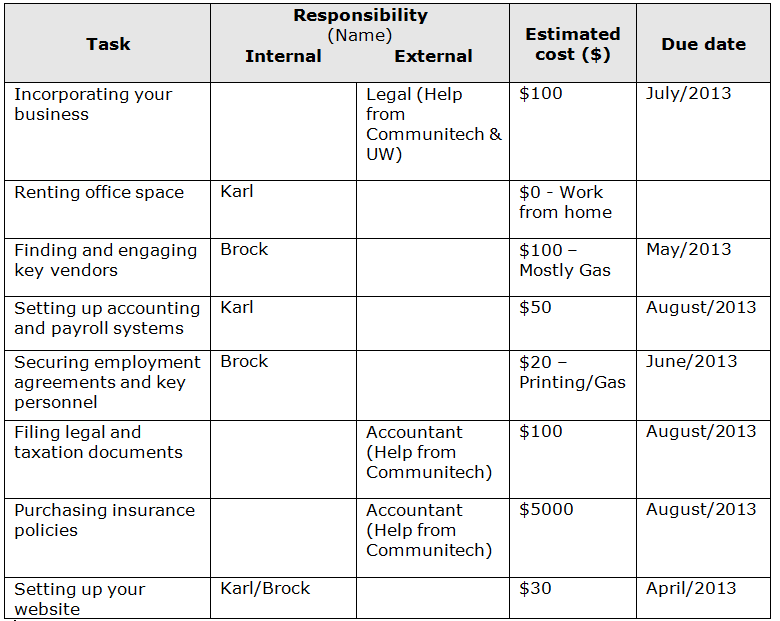
\includegraphics[width=150mm]{images/TaskList.png}
\caption{Task Breakdown}
\label{tasks}
\end{figure}

\subsection{Growth Plan}
The stepping stones described in the Go-to-Market Strategy section of the plan are reiterated in the following financing roadmap. The necessary funding required for each step is presented underneath the appropriate stepping stone.

\begin{figure}[ht!]
\centering
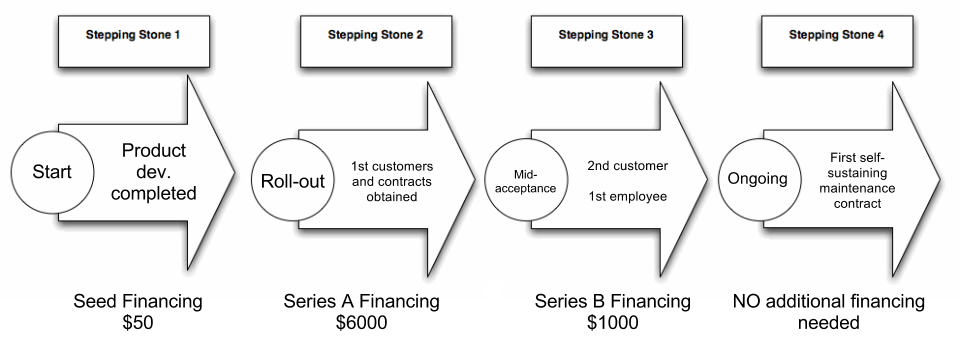
\includegraphics[width=150mm]{images/MSCI454-FinancingRoadmap.png}
\caption{Financing Roadmap}
\label{steppingStones}
\end{figure}
 
Initially only \$150 seed financing will be required. This will cover menial costs associated with working from home and developing {\it Acknowledgements}. This cost does not account for compensating founders during the initial development phase as the co-founders will not be compensated until the first clients have been established.

Series A financing entails purchasing the required server space to host our application for our client to access it before we have started to receive revenue. The rest of the costs associated with this stage of financing are associated with travel to and from client meetings.

Series B financing is again to cover small costs that have to do with client meetings. All necessary expansion costs are covered by the revenue obtained by initial client membership fees.

During the ongoing phase, {\it Acknowledgements} is self-sustaining based on revenue and does not need additional financing.

% \subsection{Pitch Scenarios}
% Ideally, you can provide two sales scenarios based on a high and low case to show the sensitivity and range for your plan.

\subsection{Accounting}
The {\it Acknowledgements} Balance Sheet for the first year is presented in the following table. This Balance Sheet does not account for the development hours worked by the founders, who will not initially be compensated for their work.

\begin{table}[ht]
\caption{The Balance Sheet} % title of Table
\centering % used for centering table
\begin{tabular}{| l | p{1in} | p{1in} | p{1in} |} % centered columns (4 columns)
\hline
{\bf Item of Service} & {\bf Cost per Unit  (\$)} &  {\bf Quantity in First Year } &  {\bf Cost for First Year (\$) } \\
\hline
 &   &   &   \\
{\bf Office (Work from home)} & & & \\
	Computers & 1,500 & 2 & 3,000 \\
	Internet Service & 60 & 12 & 720 \\
	Office Supplies & 300 & 1 & 300 \\
	Printer & 150 & 1 & 150 \\
 &   &   &   \\
{\bf Product} &   &   &   \\
	Web Hosting & 150 & 1 & 150 \\
	Development Hours (unpaid) & 0 & 750 & 0 \\
	Development Hours (paid) & 30 & 1000 & 30,000 \\
  &   &   &   \\
{\bf Client Meetings} &   &   &   \\
	Lunches & 50 &  50 & 2,500\\
	Gas & 50 & 20 & 1,000 \\
  &   &   &   \\
{\bf Legal} &   &   &   \\
	Incorporation & 300 &  1 & 300\\
	Insurance & 5,000 & 1 & 5,000 \\
 &   &  &   \\ 
{\bf Total} &   &   & {\bf 43,120} \\
\hline
\end{tabular}
\label{balanceSheet} % is used to refer this table in the text
\end{table}